\begin{figure}[h]
    \centering
    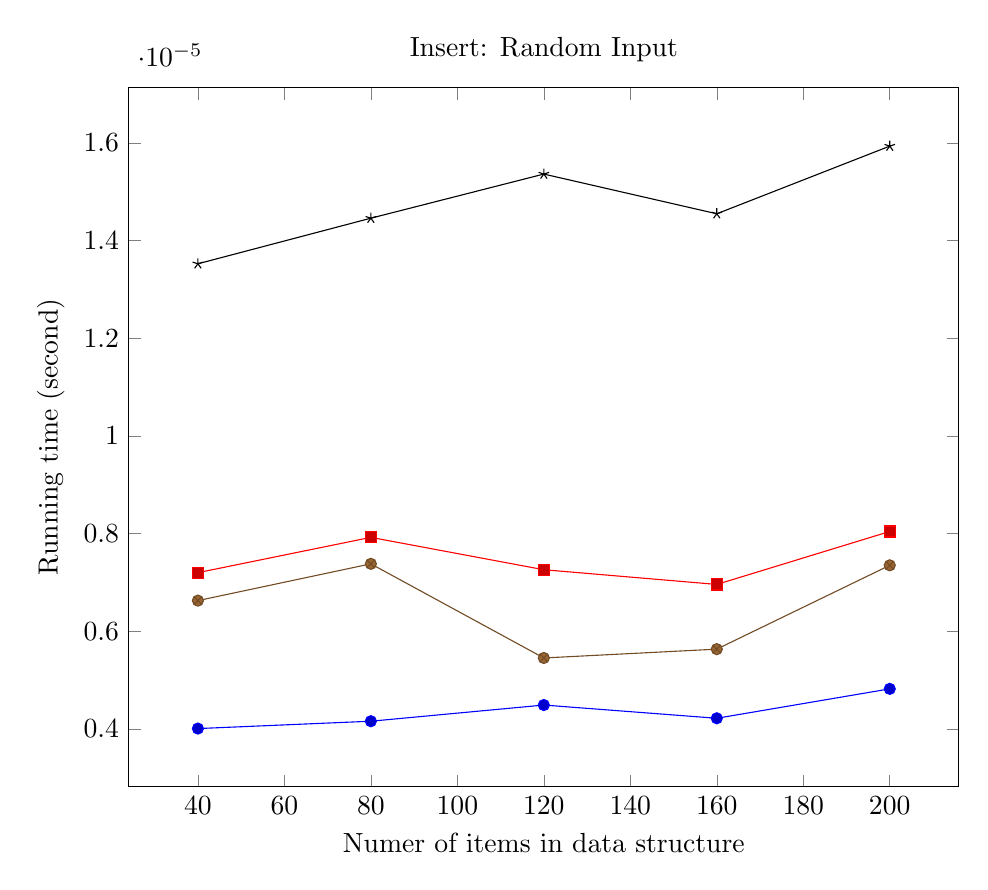
\begin{tikzpicture}
        \begin{axis}[
            xlabel={Numer of items in data structure},
            ylabel={Running time (second)},
            title={Insert: Random Input},
            width=\textwidth
        ]
		\addplot coordinates {
			(40, 4.005631978797053e-06)
			(80, 4.1562196471736645e-06)
			(120, 4.487512517599434e-06)
			(160, 4.216454714522922e-06)
			(200, 4.81880538802798e-06)
		};
		\addplot coordinates {
			(40, 7.198090548365954e-06)
			(80, 7.920911356569526e-06)
			(120, 7.258325615715211e-06)
			(160, 6.957150278963376e-06)
			(200, 8.041381491270816e-06)
		};
		\addplot coordinates {
			(40, 6.625857408536218e-06)
			(80, 7.378795750415113e-06)
			(120, 5.451273595204198e-06)
			(160, 5.631978797256132e-06)
			(200, 7.348678216741178e-06)
		};
		\addplot coordinates {
			(40, 1.3522772620150336e-05)
			(80, 1.4456416164079777e-05)
			(120, 1.5359942174335284e-05)
			(160, 1.4546768765105744e-05)
			(200, 1.5932175314163634e-05)
		};
        \legend{}
        \end{axis}
    \end{tikzpicture}
    \caption{Average of 0 operations, benchmarked every 0, starting at 0.}
\end{figure}